\documentclass[10pt, conference, compsocconf]{IEEEtran}
\usepackage{float}
\usepackage{hyperref}
\hypersetup{
	colorlinks=true,
	linkcolor=black,
	citecolor=black,
	urlcolor=blue,
}
\usepackage{fullpage}
\usepackage{graphicx}
\usepackage{color}
\usepackage{setspace}
\usepackage{subfigure}
\usepackage{algorithm, algorithmic}
\usepackage{multirow}
\usepackage[table]{xcolor}
\usepackage{url}
\usepackage{cite}
\usepackage{fancyvrb}
\usepackage{amsmath, amsfonts}
\usepackage{rotating}
%% To help with graphics importing.
\usepackage{graphicx}
\usepackage{color}
\DeclareGraphicsRule{.pdftex}{pdf}{*}{}
\graphicspath{{figures/}}

% InputFigure
% This command is just a wrapper around \input, to abstract out the path
% and extension of figures.  We're using PDFTeX to make sure that fonts
% are handled correctly from the beginning.
% #1: Filename, without extension or directory.
\newcommand{\InputFigure}[1]{
	\input{figures/#1.pdftex_t}
}

\newcommand{\InputPlot}[1]{
	\includegraphics{#1}
}

%% Some helpful lengths.
\newlength{\HalfPage}
\setlength{\HalfPage}{0.45\textwidth} % <.5, so that we can pack figures side-by-side.
\newlength{\OneColumn}
\setlength{\OneColumn}{0.45\textwidth}

%% New commands; short ones go here.
\newcommand{\dk}[1]{\emph {[[dk: #1]]}}

\newcommand{\mysection}[1]{\section{#1}}
\newcommand{\mysubsection}[1]{\subsection{#1}}

\newcommand{\term}[1]{{\em #1}}
\newcommand{\etal}{{et al.}}
\newcommand{\selfstar}{{\em self-}$\ast$}

\newcommand{\coreworld}{\sc Core~World}
\newcommand{\tierra}{\sc Tierra}
\newcommand{\avida}{A{\sc vida}}
\newcommand{\neat}{NEAT}
\newcommand{\hyperneat}{HyperNEAT}
\newcommand{\multiagent}{Multi-agent HyperNEAT}
\newcommand{\boldavida}{\bf {A\small{VIDA}}}
\newcommand{\instr}[1]{{\sc #1}}
\newcommand{\task}[1]{{\sc #1}}
\newcommand{\event}[1]{{\sc #1}}
\newcommand{\code}[1]{{\sf #1}}

\newcommand{\CalloutAlg}[1]{Algorithm~\ref{#1}}
\newcommand{\CalloutTable}[1]{Table~\ref{#1}}
\newcommand{\CalloutFigure}[1]{Figure~\ref{#1}}
\newcommand{\CalloutChapter}[1]{Chapter~\ref{#1}}
\newcommand{\CalloutSection}[1]{Section~\ref{#1}}
\newcommand{\CalloutEqn}[1]{Equation~\ref{#1}}


%% These are weird...

%%%%%%%%%%%%%%%%%%%%%%%%%%%%%%%%%%%%%%%%%
%
% USAGE: \begin{bfigure}{pos}{wid} text \end{bfigure}
%    pos    the usual figure placement arg: eg. htbp (p.176,latex)
%    wid    the width of the figure, in some units: eg. 5in
%    text   the contents of the figure, including picture/caption/label/etc
%*%  Should steal code from LaTeX to make the interface the same (e.g.
%*%  with `htbp' in braces [] instead of an argument)
\newenvironment{bfigure*}[2]{
    \begin{figure*}[#1]
\centering
\begin{bbox}{#2}
    }{
\end{bbox}
    \end{figure*}
}

%%%%%%%%%%%%%%%%%%%%%%%%%%%%%%%%%%%%%%%%%
% BBOX environment
%%%%%%%%%%%%%%%%%%%%%%%%%%%%%%%%%%%%%%%%%
%
\newenvironment{bbox}[1]{
    \begin{tabular}{|p{#1}|} \hline
}{\\ \hline
    \end{tabular}
}
\newcommand{\spa}{\hspace{1ex}}
\newcommand{\spb}{\hspace{2ex}}


% A ``monkey'' figure function - does it all.
% #1: Width
% #2: Rotate
% #3: Label (filename)
% #4: Caption
\newcommand{\Figure}[4]{
	\begin{figure}[h]
	\center
	\resizebox{#1}{!}{
	\rotatebox{#2}{\includegraphics{figures/#3}}}
	\caption{#4}
	\label{#3}
	\end{figure}
}

\newcommand{\GetFigure}[2]{
	\resizebox{#1}{!}{
	\includegraphics{figures/#2}}
}	

% size
% before skip
% after skip
% figure
% caption
%\newcommand{\FigureSkip}[5]{
%	\begin{figure}[h]
%	\center
%	\vspace{#2}
%	\resizebox{#1}{!}{
%	\includegraphics{figures/#4}}
%	\vspace{#3}
%	\caption{#5}
%	\label{#4}
%	\end{figure}
%}

% Figure start; useful with \SubFloat
%\newcommand{\FigureBegin}{
%	\begin{figure}[htp]
%	\centering
%}

% Figure end; useful with \SubFloat
% #1: Label of whole figure
% #2: Caption of whole figure
%\newcommand{\FigureEnd}[2]{
%	\caption{#2}
%	\label{#1}
%	\end{figure}
%}

% A sub-float; useful with \Figure{Begin/End}
% #1: Width
% #2: Filename
% #3: Caption
%\newcommand{\Subfloat}[3]{
%	\subfloat[#3]{\label{#2}\includegraphics[width=#1]{figures/#2}}
%}

% should eventually save this...
%\floatstyle{boxed}
%\newfloat{program}{thp}{lop}
%\floatname{program}{Program}
%\floatstyle{plain}

%\newcommand{\choose}[2]{\left(\begin{array}{c}#1\\#2\end{array}\right)}

% For including large-ish program fragments.
% #1: Width (not scaled)
% #2: Label (filename)
% #3: Caption
%\newcommand{\Program}[4]{
%	\begin{figure}[htb]
%	\center
%	\lstset{linewidth=#1}
%	\lstset{frame=lrtb}
%	\lstinputlisting[caption=#3,label=#2]{figures/#2}
%	\end{figure}
%}


\begin{document}
\sloppy

\title{TBD}

\author{\IEEEauthorblockN{David B.~Knoester and others}
\IEEEauthorblockA{Dept.~of Microbiology and Molecular Genetics\\
Michigan State University\\
East Lansing, Michigan 48824\\
Email: \{dk\}@msu.edu}}
\maketitle

\begin{abstract}
Combining systems that self-organize with those that self-adapt is an important problem in SASO systems.  In thi
An important problem in self-organizing and self-adaptive systems is how to merge 
%This paper describes a study in the use of neuroevolution to discover controllers for a simulated mobile ad hoc network.  Neuroevolution is a technique whereby an evolutionary algorithm is used to produce artificial neural networks that solve a user-defined task.  Here, we use neuroevolution to study a generic coverage-based problem, where agents in the network are to maximize the area covered by the largest connected component of the network.  An example application for this work is the discovery of control algorithms for an ocean-monitoring mobile network.  While this is a challenging problem domain for neuroevolution, results of our experiments reveal three important characteristics to be considered when using such an approach.  Specifically, we found that approaches that implicitly reduce entropy, while explicitly addressing self-organization and scalability, are capable of discovering behaviors that remain stable even when they control networks of different sizes than were evaluated during evolution.  This result suggests that neuroevolution may be a viable strategy for discovering controllers for self-organizing multi-agent systems.
\end{abstract}

\begin{IEEEkeywords}
Evolutionary algorithm, cellular automata, self-organization, self-adaptation.
\end{IEEEkeywords}

%!TEX root = main.tex
\section{Introduction}\label{s:intro}

Nature provides us with many examples of self-organizing systems, from inorganic X to the wondrously complex behavior of social organisms such as honeybees, ants, and even larger mammals~\cite{?}.  In addition to being self-organizing, many natural systems are also {\em self-adaptive}, where the agents within each system change their behavior over time, in response to environmental stimuli.  Learning is one such example of a self-adaptive behavior.  While many researchers have taken inspiration from self-organizing biological systems to develop self-organizing computational systems, few have demonstrated systems that are both SO and self-adaptive.  Indeed, it remains a challenge to show how SO and SA systems might be merged into a unified framework to enable us to engineer the next generation of large scale distributed computing systems.

To further our understanding of such systems, researchers have long relied upon ``simple'' mathematical models or simulations.  Among these model systems are the well-known {\em cellular automata}, in which cells in a typically grid-structured environment follow simple rules to update their state.  The well-known ``Game of Life''~\cite{conway} is one such example of a 2-dimensional elementary cellular automata.  The behavior of a typical CA can be completely described by a set of rules $\Phi$, which is simply a binary vector containing a single entry (the output state) for each of the possible states of a given cell's neighborhood.  Depending on the dimension of the CA and the radius of a cell's neighborhood, rule sets can be either very simple, or unimaginably large and complex.

Many different approaches to discovering the ruleset for a CA have been devised.  While some rely upon enumeration of all possible rulesets, others have employed various search techniques to discover rulesets that solve a given problem.  For example, Mitchell~\etal have demonstrated that genetic algorithms are capable of discovering 128-bit rulesets that solve the 1D, n=35, r=3 majority bit and synchronization problems.  Others, using different EAs, have shown interesting relationships between rulesets and CA topology~\cite{?}.  While these approaches to CAs have already shed light on many of the principles behind SO systems, they do not address systems that include an ability to self-adapt.

In this paper, we focus on cellular automata that {\em both} self-organize and self-adapt.  We use a novel evolutionary algorithm that is able to construct adaptable state machines to solve the CA bit-consensus problem.  We demonstrate that these state machines are able self-organize and solve the bit-consensus problem in 1-, 2- and 3-dimensional CAs in a scale-free manner.  Finally, we show that the addition of a global reinforcement signal dramatically improves the evolvability and performance of this system, and that such a signal confers a high degree of resilience to environmental perturbation.

The contributions of this work are as follows.  First, we present one method by which self-organizing and self-adaptive systems can be discovered.  Second, we demonstrate the effectiveness of this approach on 1-, 2-, and 3-dimensional cellular automata, and show that the solutions discovered by an evolutionary algorithm scale to CAs many times their evolved size.  Finally, we show howl the combination of an adaptive system with global reinforcement signals provides a high degree of resilience to environmental perturbation.  These results support the use of cellular automata based systems as a study system for exploring SASO principles, show one method by which self-adaptation can be included in self-organizing systems, and further strengthen the case for the use of evolutionary algorithms to discover SASO systems.
%!TEX root = main.tex
\section{Related Work}\label{s:related}
%Traditionally a subfield of distributed artificial intelligence, {\em distributed problem solving} is the use of multiple, semi-autonomous, and cooperating agents to solve a problem~\cite{weiss1999multiagent}.  Occasionally, a distinction is drawn between decomposition/distribution approaches, and those that rely on autonomous interactions among agents, known as multi-agent systems (MAS)~\cite{panait2005cooperative}.  The task of controlling the formation of a group of agents has been examined from different perspectives, including graph-stability, switching hierarchical control strategies, adaptive gradient climbing, and others~\cite{cassandras2005sensor}.  Here, instead of {\em engineering} control algorithms for the movement of agents, we employ neuroevolution to automatically {\em discover} controllers for a mobile network.
%
%In the broader context of MAS, the taxonomy provided by Panait and Luke~\cite{panait2005cooperative} places our study in the {\em team learning} category, where a single evolving individual encodes the behavior for the entire team (mobile network, in this case).  Moreover, the agents in this study engage in {\em direct communication} through message-passing, and no mechanism for indirect communication (e.g., stigmergy) is provided.  Finally, the scenario that we have selected for study is related to {\em cooperative target observation}, where a group of agents is tasked with collective observation of a target.  The specifics of our scenario will be explained in more detail in \CalloutSection{s:methods}.
%
%Within evolutionary computation, numerous techniques have been proposed to evolve cooperative teams that solve tasks. Waibel, Keller, and Floreano survey the work done in this area~\cite{waibel2009genetic}. Their classification highlights whether the group is homogeneous or heterogeneous and whether selection is performed at the level of the individual or team.  Additionally, they compare the performance of four types of teams: (1) homogeneous teams using individual selection; (2) homogeneous teams using group selection; (3) heterogeneous teams using individual selection, and (4) heterogeneous teams using group selection, on four cooperative tasks. Their results indicate that the genetic composition of groups and level of selection are key factors in evolving groups that perform cooperative tasks, and in general, find that homogeneous teams, as used here, tend to outperform other approaches.
%
%Neuroevolution is a kind of evolutionary algorithm that evolves ANNs.  {\neat} (NeuroEvolution of Augmenting Topologies)~\cite{stanley2002evolving}, described in more detail in \CalloutSection{s:methods}, has previously been used to evolve teams of agents through real-time interaction with a player, where each agent was controlled by an instance of an evolved neural network~\cite{stanley2005real}.  Neuroevolution has also produced adaptive teams, where agents with identical neural networks nonetheless exhibit different behaviors~\cite{bryant2003neuroevolution}.  Our study leverages {\neat} to address problems in the control of MANETs.
%
%Quint\~{a}o, Nakamura, and Mateus~\cite{quintao2005evolutionary} have studied dynamic coverage problems, and used an evolutionary algorithm to optimize the coverage of sensors set in fixed locations.  Hauert, Zufferey, and Floreano~\cite{hauert2009evolved} have also studied the use of a neural network controller for unmanned aerial vehicles (UAVs), where the ANN was evolved via a genetic algorithm.  Here, the UAVs were to establish and maintain a multi-hop communications link between a base station and a target without global or agent-relative positioning information.  Finally, D'Ambrosio {\etal}~\cite{dambrosio2010evolving} investigated the use of derivatives of {\neat} on a coverage-based problem, where agents were able to sense the boundaries of their environment, but were not able to sense other agents.  In the study presented here, we investigate the control of agents that are able to sense their positions in an open environment, but yet must coordinate to solve a coverage-related problem.
%
%In a previous study, we used a variety of different neuroevolutionary approaches to discover neural network controllers for nodes in a MANET~\cite{knoester2010neuroevolution}.  The main result of our prior study was that, regardless of the specific neuroevolutionary approach, the difficulty of controlling the network increased with the number of nodes.  In the study presented here, we again use neuroevolution to discover controllers for a MANET.  However, here we focus on one neuroevolutionary system, {\neat}, and propose solutions to three different aspects of this problem that were previously found to be challenging: network stability, self-organization, and scalability.
%
%
%%here we propose three characteristics that should be exhibited by large-scale systems:  First, the system must be {\em predictable}, which is to say that we as engineers should have confidence that the behavior of the system matches our expectation.  Second, the system must be {\em self-organizing} -- It cannot rely on the presence (or correct operation) of a central coordinator.  Finally, the system must be {\em scalable}.  Though self-organization and scalability are often correlated with each other in nature, in this study we treat them as separate aspects of behavior.  The question we address in this study is then, ``How can we discover behaviors distributed systems that are predictable, self-organizing and scalable?''
%
%%Specifically, we evaluated multiple variations of three different neuroevolutionary systems ({\neat}~\cite{stanley2002evolving}, {\hyperneat}~\cite{stanley2009a-hypercube-based}, and {\multiagent}~\cite{dambrosio2008generative}) on a coverage problem, where the agents were required to distribute themselves on a grid while maintaining network connectivity.  Each of these systems was used to evolve one or more artificial neural networks (ANNs), which were used as controllers for both the movement and communication behavior of agents within the network.  This problem thus includes not only a functional component (i.e., ``spread out to cover a region''), but also a non-functional component related to the topology of the network.  Agents were provided with simulated radios, and were able to broadcast to their neighbors within a limited range.  Whether agents were able to communicate with each other was defined by whether a neighbor is transmitting and also by distance between individuals.

%!TEX root = main.tex
\section{Methods}\label{s:methods}


Traditional evolutionary algorithms (EAs) encode the biological process of evolution by natural selection in software so that they can be used to search for solutions to complex, high-dimensional problems~\cite{Eiben:2003tf}.  For example, the well-known genetic algorithm has been used to solve a wide-variety of engineering optimization problems~\cite{Goldberg:1989uj}, while genetic programming has consistently produced human-competitive results in fields as diverse as circuit layout and antenna design~\cite{Koza:2005wg,Lohn:2004to}.

{\em Markov Network Brains} (MNBs) are probabilistic automata that can be evolved via genetic algorithms~\cite{Edlund:2011kt}.  MNBs comprise a series of {\em gates}, where each gate accepts input and produces output, much like a neuron in an artificial neural network.  Each gate is itself governed by an evolved truth table.  
%
These truth tables may be binary, in which case the corresponding gate implements a small logic circuit, as shown in Table~\ref{t:logic-gate}.  Gates may also be probabilistic, in which case the evolved truth table contains probabilities, as shown in Table~\ref{t:prob-gate}.  In all cases, input to and output from evolved gates are binary.  Gates are subject to mutation, which may alter the fan-in or fan-out of the gate, or ``rewire''  the gate to connect an input or output to a different {\em state variable}, which provide input, output, or hidden states to the entire MNB, as shown in Figure~\ref{f:mnb-example}.

\begin{table}[h]
    \centering
    \caption{Example truth table for an evolved logic gate.  $X$ and $Y$ are binary inputs, $Z$ is a binary output.  This truth table implements the logic function $Z=X \lor \lnot Y$, which highlights the ability of evolution to use non-standard logic functions.}
    \begin{tabular}{ll|l}
    \hline
        {\bf X} & {\bf Y} & {\bf Z} \\\hline
        0 & 0 & 1\\
        0 & 1 & 0\\
        1 & 0 & 1\\
        1 & 1 & 1\\
        \hline
    \end{tabular}
    \label{t:logic-gate}
\end{table}

\begin{table}[h]
    \centering
    \caption{Example truth table for an evolved probabilistic gate.  $X$ and $Y$ are binary inputs, $Z$ is a binary output.  The output ($Z$) of this gate is given as a probability based on the combination of inputs $X$ and $Y$.  For example, $P(Z=1)$ given $X=1$ and $Y=1$ is 0.25.}
    \begin{tabular}{ll|ll}
    \hline
        {\bf X} & {\bf Y} & {\bf P(Z=0)} & P(Z=1) \\\hline
        0 & 0 & 0.0 & 1.0\\
        0 & 1 & 0.95 & 0.05\\
        1 & 0 & 0.5 & 0.5\\
        1 & 1 & 0.25 & 0.75\\
        \hline
    \end{tabular}
    \label{t:prob-gate}
\end{table}

\begin{figure}
\centering
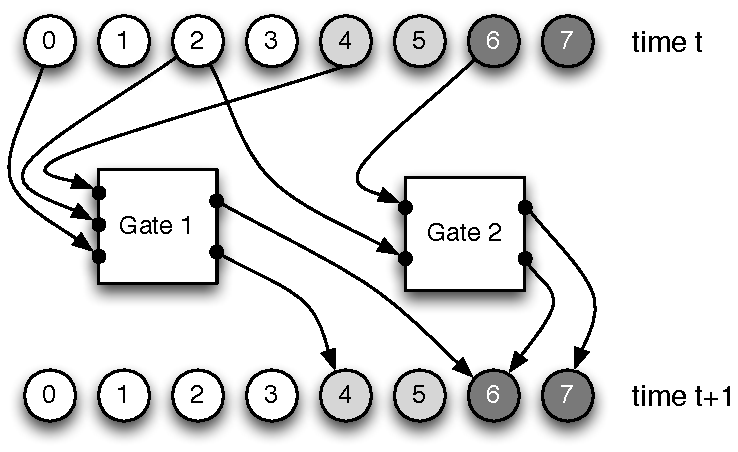
\includegraphics[width=0.45\textwidth]{markov-network-example}
\caption{An example Markov Network Brain (MNB) with 12 state variables: Four input states (white circles, 0-3), two hidden states (light grey circles, 4 and 5), two output states (dark grey circles, 6 and 7), and two gates (white squares, ``Gate 1" and ``Gate 2"). The MNB receives input in states 0-3 at time $t$, then each gate is activated, and their respective outputs are written into states 4, 6, and 7 at time $t+1$.}
\label{f:mnb-example}
\end{figure}

Figure~\ref{f:mnb-genome} depicts the {\em genome} for a MNB.  This genome is typically a circular list of integers ({\em codons}) that contains a series of {\em genes}.  Each gene encodes a single gate, and defines that gate's fan-in, fan-out, truth table, and the mapping of inputs and outputs to state variables.  The beginning of a gene is indicated by a {\em start codon}, a specified sequence of two integers, and the extent is determined by the size of the corresponding gate's truth table.  The entire genome is subject to mutation, including point-mutations (i.e., replacing a codon with a random integer), insertions (i.e., inserting a random sequence into the genome),  and deletions (i.e., deleting a random sequence from the genome).

\begin{figure}
\centering
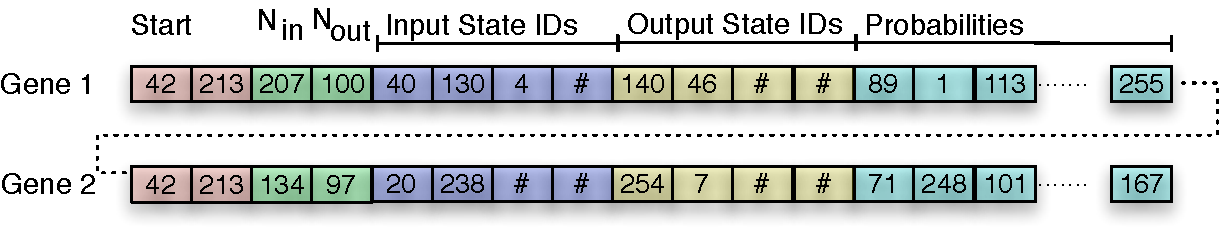
\includegraphics[width=.45\textwidth]{markov-network-genome}
\caption{Example genome containing two genes. The sequence (42, 213) is the start codon, and represents the beginning of a gate(red blocks). The next two codons describe the fan-in and fan-out of the gate (green blocks), and the following eight codons map inputs (blue blocks) and outputs (yellow blocks) to state variables.  The remaining codons comprise the gate's truth table (cyan blocks).}
\label{f:mnb-genome}
\end{figure}

While MNBs have most frequently been used to evolve controllers for agents in embedded environments~\cite{Edlund:2011kt,Olson:2013kx,Olson:2013ko}, we have recently begun applying MNBs to problems in engineering, specifically optical character recognition~\cite{Chapman:2013kf} and time-series forecasting (manuscript in preparation).  
%
MNBs have shown a remarkable ability to model state transitions that underlie a noisy physical process, as shown in Figure~\ref{f:mnb-model}.  Here, we will evolve MNBs to examine time-series data for abnormalities that are indicative of cancer.

\begin{figure}
\centering
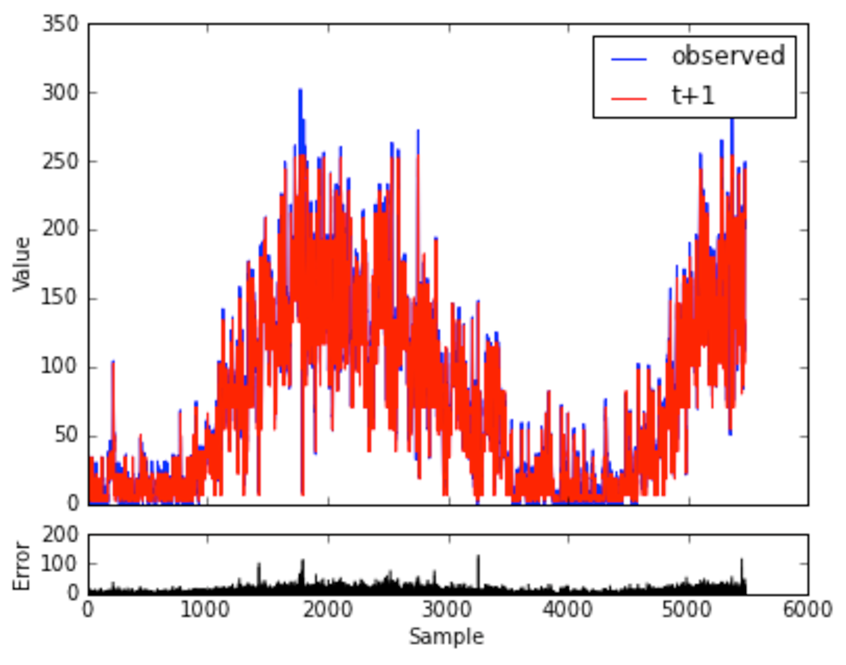
\includegraphics[width=.45\textwidth]{markov-network-sunspot}

\includegraphics[width=\textwidth]{markov-network-graph}
\caption{These figures show preliminary results of using MNBs to forecast space weather, specifically the daily number of sunspots visible from Earth.  This data is highly chaotic, and has a prediction horizon of 8 days.  At top we see a comparison of daily predicted vs.~observed sunspot numbers for the time period 1975 to 1989; at bottom is a depiction of the MNB that evolved to predict this time series.  These results indicate that MNBs are highly effective at time-series analysis.}
\label{f:mnb-model}
\end{figure}





%This section describes the neuroevolutionary approach and the specific problem we addressed in this study.

% cellular automata
% traditional rule encoding, vis a vis game of life
% FSM rules
% PSM rules
% PSM adaptation
% evolutionary algorithm & FSMs/PSMs
% -- all parameters found online?

%
%\begin{figure}
%\centering
%\subfigure[]{\label{f:complex-frame0}\includegraphics[width=\HalfPage]{frame0001}}
%\hspace{1em}
%\subfigure[]{\label{f:complex-frame1}\includegraphics[width=\HalfPage]{frame0164}}
%\caption{Starting configuration of agents~\subref{f:complex-frame0} and position of agents 4s into a simulation~\subref{f:complex-frame1}.  White lines represent connections between agents; agents can transmit data only to those other agents to which they are connected.  The grid agents are to cover is outlined with black lines; $x$, $y$, and $z$ axis represented by red, green, and blue lines, respectively.}
%\label{f:grid-coveragea}
%\end{figure}
%
%\begin{table}[h]
%\centering
%\caption{Sensors and effectors of individual agents for the grid-coverage problem.}
%\label{t:agent}
%\begin{tabular}{ll p{11em}}
%\hline\hline
%Name & Type & Description\\\hline
%\code{rx0}\ldots\code{rx3} & sensor & directional radio receiver; each sensor covers a 90$^\circ$ ``pie slice'' around the agent\\
%\code{v0}\ldots\code{v2} & sensor & velocity vector $(x,y,z)$\\
%\code{p0}\ldots\code{p2} & sensor & absolute position $(x,y,z)$\\
%\code{f0}\ldots\code{f2} & effector & force vector $(x,y,z)$\\
%\code{tx} & effector & broadcasts a message to all agents within range; appropriate \code{rx} sensor is always set to the inverse of the distance between sender and receiver\\\hline
%\end{tabular}
%\end{table}

%\begin{table}[htb]
%\centering
%\caption{Relevant configuration parameters for {\neat}; those not listed are set to their default value.}
%\label{t:neat}
%\begin{tabular}{l l}
%\hline\hline
%Parameter & Value\\\hline
%PopulationSize & 100\\
%MaxGenerations & 200\\
%MutateAddNodeProbability & 0.03\\
%MutateAddLinkProbability & 0.05\\
%MutateDemolishLinkProbability & 0.03\\
%MutateLinkWeightsProbability & 0.8\\
%MutateOnlyProbability & 0.25\\
%MutateLinkProbability & 0.1\\
%AllowAddNodeToRecurrentConnection & 1.0\\
%AllowRecurrentConnections & 0.0\\
%AllowSelfRecurrentConnections & 0.0\\
%OnlySigmoidHiddenNodes & 1.0\\\hline
%\end{tabular}
%\end{table}
%
%
%

%!TEX root = main.tex
\section{Experiments and Results}\label{s:results}

%In this section, we present our experiments and results on using {\neat} to evolve neural network controllers for the nodes in a mobile ad hoc network.  When evaluating a given ANN, nodes in the simulation shared the same neural network structure (neurons, links), but had their own instance of the neural network -- It may be helpful to think of a MANET as a single homogeneous population of neural networks.  In all of the experiments presented below, we require that the network: (1) be connected at the time of fitness evaluation, and (2) that the centroid of the network less than 200m from the origin, otherwise the minimum possible fitness is assigned to that individual (note that it may still be selected for recombination, though this is unlikely).  These steps were optimizations to reduce computation time.


%%%%
%\subsection{Motivating Experiment}\label{s:baseline}
%Our first experiment investigated the evolution of neural networks that could solve the grid-coverage problem, and it provides the motivation for the following experiments.  Specifically, the fitness function used here was simply that shown in \CalloutEqn{e:grid-coverage}, which was evaluated after 10s of simulation time.
%
%\CalloutFigure{f:1-fixed-network} plots the mean normalized fitness of the dominant (most fit) individual per generation across 30 separate trials for both 8-node ($FF8$) and 16-node ($FF16$) networks.  The (very small) error bars in this and other figures are 95\% confidence intervals constructed via 200-fold bootstrapping.  We define {\em normalized fitness} as $f/f_{max}$, where $f_{max}$ is the maximum possible fitness achievable given the fitness function and network size.  In this treatment, fitness and normalized fitness are identical, although that is not the case in many of the following experiments.  In \CalloutFigure{f:1-fixed-network}, we see that the dominant individuals in 8-node networks reach their optimal fitness after approximately 40 generations, while 16-node networks averaged only $71.5\pm0.6$\% after 200 generations.
%%(We note that fitness calculation is slightly different [10s as opposed to here than in previous experiments, thus these results are not exactly the same as in \CalloutSection{s:results-complex}.)
% 
%\begin{figure}[htb]
%\centering\includegraphics[width=\HalfPage]{1-fixed-network}
%\caption{Normalized fitness of 8- and 16-node fixed-size networks using a fitness function that rewards only for grid-coverage.}
%\label{f:1-fixed-network}
%\end{figure}
%
%Upon examination of the evolved behaviors, the reason for the decline in fitness of 16-node networks became apparent: For both 8- and 16-node networks, the evolved strategies were primarily stochastic, and relied upon the continual movement of nodes throughout the environment.  One such behavior is depicted in \CalloutFigure{f:2-fixed-movement}, which shows the position and velocity vectors of each node in the 16-node network over 20s of simulation time.  In this figure, nodes start in an array along the $x-$axis, and generally move in a spiral pattern within the region bounded by the grid.  A movie of this behavior (and others described in the following sections) is available at: \url{http://www.cse.msu.edu/thinktank/manet}.  This behavior was also prevalent in the smaller 8-node networks.  The reason this strategy is effective is related to the size of the grid relative to the number of nodes in the network.  On average, if the grid is large relative to the size of the network, and nodes maintain some distance between each other while moving over the grid, nodes are likely to be in different cells at the time of fitness evaluation.  This strategy is less effective with larger MANETs because nodes are more likely to occupy the same cell.  Interestingly, this strategy is not unlike that exhibited in flocks of starlings~\cite{fernandez-juricic2004flock}, where individuals adjust their movements to maintain a ``safe'' distance amongst themselves.
%
%\begin{figure}[htb]
%\centering\includegraphics[width=\HalfPage]{2-fixed-movement}
%\caption{Sample velocity and position of a 16-node network following 20s of control ($FF16$ treatment).  Nodes start at $(x,0)$, and then move in a spiral for the remainder of the simulation.}
%\label{f:2-fixed-movement}
%\end{figure}
%
%However, from the perspective of engineering controllers for a MANET, these evolved behaviors are lacking in two significant ways: First, the evolved behaviors are {\em unstable}.  We expected to see behaviors where nodes would deterministically move to unique cells in the grid and stop moving.  Instead, the nodes moved continually in a spiral pattern, which would waste energy in a real network.  Second, these behaviors do not {\em scale}.  We hoped to evolve effective behaviors for networks of varying size.  However, we found that normalized fitness decreased as network size increased, a result which we verified on larger 32-node networks and both larger and smaller grids.  In all cases, the key factor was the number of nodes being controlled, which is known to be a challenge for multi-agent systems~\cite{panait2005cooperative}.  In the following experiments, we examine ways to improve network stability and scalability.
%
%
%%%%%
%\subsection{Stable Networks}\label{s:speed}
%Based on the behaviors observed in the previous experiment, we first explored ways to improve network stability.  The goal here was to discover networks whose nodes would move to and then settle in a location, instead of continuing to move throughout the environment.  Our first approach was to devise a fitness function that included a speed component, such that networks with nodes that were moving slowly at the time of fitness evaluation would have a higher fitness than a network whose nodes were moving quickly.  This fitness function, $SF(M)$, rewarded for a reduction in the average speed at which nodes in $M$ (the MANET) were moving, specifically:
%%
%\begin{equation}
%SF(M) = \frac{G(M,36)}{10\cdot\max(0.1, \overline{\mathrm{spd}(M)})}
%\label{e:sf}
%\end{equation}
%%
%where $G(M,36)$ is performance on the 36-cell grid-coverage problem, and $\overline{\mathrm{spd}(M)}$ is the average speed of all nodes in $M$ at the end of the simulation.  The other components of this fitness function, scaling by 10 and $\max(\cdot)$, were used to ensure that the resulting fitness score is in the range $[0..1]$.  This fitness function thus rewards MANETs that quickly move to, and settle, in a stable configuration.
%
%\CalloutFigure{f:3-slow-network} plots the mean normalized fitness of the dominant individual per generation over 30 trials on networks of 16 nodes.  Surprisingly, the mean normalized fitness of dominant individuals under this treatment is $55.3\pm1.2$\% after 200 generations, which is even worse than in the base $FF16$ case.  Upon examination of the evolved behaviors, however, we did indeed find that the networks exhibited the desired behavior, where nodes stabilized into a fixed position after reaching their target cells, although many nodes shared occupancy of cells.
%
%\begin{figure}[htb]
%\centering\includegraphics[width=\HalfPage]{3-slow-network}
%\caption{Normalized fitness for 16-node networks that are rewarded for reduced speed.}
%\label{f:3-slow-network}
%\end{figure}
%
%%Upon examination of the evolved behaviors, we did indeed find that the networks exhibited the desired behavior, where nodes stabilized into a fixed position after reaching their target cells.  An example of this behavior is shown in \CalloutFigure{f:4-slow-movement}, which shows the position and velocity of each node during 20s of simulation time.  Nodes again start in an array along the $x-$axis, and slowly move to different grid cells, although many nodes share cells.%  A video of this behavior is available at: \url{http://somewhere-else}.
%
%%\begin{figure}[htb]
%%\centering\includegraphics[width=\HalfPage]{4-slow-movement}
%%\caption{Velocity and position of 16 nodes in the network evolved under treatment $SF16$, which rewards for a reduction in the average speed of nodes at the end of the simulation.}
%%\label{f:4-slow-movement}
%%\end{figure}
%
%%%%%
%\subsection{Reducing Entropy}\label{s:redentropy}
%One key difference we noticed between this behavior and that shown in \CalloutFigure{f:2-fixed-movement} is that here the behavior of individual nodes was based on their starting location in the environment, and did not appear to be stochastic.  {\em Information entropy} is frequently used to characterize stochastic processes~\cite{shannon1948a-mathematical}.  To measure information entropy, $H(X)$, of a mobile network, we leverage the following definition:
%%
%\begin{equation}
%H(X) = -\sum_{i=1}^{n}p(x_{i})\log_{2}p(x_{i})
%\label{e:entropy}
%\end{equation}
%%
%where $X=\{x_{1}, \dots, x_{n}\}$ is the discrete random variable representing the states of the network, and $p(\cdot)$ is the probability mass function of $X$.  We define the states of $X$ based on the cells of the grid occupied by nodes in the network.  Specifically, each possible value of $X$ is a length-$k$ bitstring, where $k$ is the number of cells in the grid (36, in this study).  A ``1'' at position $i$ in this bitstring represents that cell $i$ is occupied by at least one node, while a ``0'' indicates that cell $i$ is not occupied.  The frequencies of these states during a simulation defines $p(\cdot)$.  Intuitively, a high value for information entropy represents a network that exhibits many states with low frequency, while a low value represents a network that exhibits few states with high frequency.  We assume that low information entropy is a desirable property of engineered systems.  For brevity, in the remainder of this paper we will refer to this calculation as the {\em entropy} of a network.
%
%\CalloutFigure{f:5-entropy} plots the mean entropy for the dominant individuals per generation over all 30 trials for two treatments: $FF16$, described in \CalloutSection{s:baseline}, whose fitness function did not include a velocity component; and $SF16$, described in this section, where a reward for reduced velocity was included as part of fitness.  As would be expected, here we see that entropy of the $SF16$ treatment is significantly lower than that of the $FF16$ treatment, indicating a more stable behaviors.
%
%\begin{figure}[htb]
%\centering\includegraphics[width=\HalfPage]{5-entropy}
%\caption{Entropy on 16-node networks under a treatment rewarding only for grid-coverage ($FF16$) and the grid-coverage plus reduced velocity ($SF16$).}
%\label{f:5-entropy}
%\end{figure}
%
%To further explore the relationship between entropy and behavior, we also devised a fitness function that rewarded explicitly for a reduction in entropy, with no consideration given to speed.  Though their performance on the grid-coverage problem was similar, the evolved behaviors were markedly different.  Specifically, when using a fitness function that rewarded for reduced entropy instead of average speed, nodes were likely to start by moving very slowly, but then would accelerate as the simulation progressed, eventually moving off the grid (data not shown).  For this reason, our subsequent experiments include speed-reduction, which implicitly reduces entropy, as a component of fitness.%, instead of an explicit reward for reduced entropy
%
%% -- In other words, while we consider low entropy to be a desirable characteristic, 
%%
%%while we consider low entropy to be a desirable characteristic, 
%%
%%our subsequent experiments include speed-reduction as a component of fitness instead of an explicit reward for reduced entropy.
%
%%\begin{figure}[htb]
%%\centering\includegraphics[width=\HalfPage]{6-entropy-movement}
%%\caption{Velocity and position of 16 nodes in a network evolved a treatment that rewarded for a reduced entropy explicitly; nodes did not stabilize into a fixed position, instead moving off the grid.}
%%\label{f:6-entropy-movement}
%%\end{figure}
%%
%%While we found that rewarding for reduced speed improved both stability and entropy of the evolved behaviors, we also noticed that these behaviors were {\em static}; that is, individual nodes no longer reacted to the presence (or absence) of neighboring nodes.
%
%%The second treatment, $EF8$, included entropy directly as part of the fitness function.  Specifically:
%%%
%%\begin{equation}
%%EF8(M) = G_{8}(M) + \frac{1}{\clip(H(M), 1, 10)}
%%\label{e:ef8}
%%\end{equation}
%%%
%%where $EF8(M)$ is fitness; $G_{8}(M)$ is again performance on the grid-coverage problem; and $H(M)$ is the entropy of the MANET calculated according to \CalloutEqn{e:entropy}, clipped to the range $[1.0, 10.0]$ to ensure that the contribution of entropy to fitness was of an equivalent range as performance on the grid-coverage problem.
%%
%%\CalloutFigure{f:sf8-ef8} contains plots of the results of these two treatments, again showing mean fitness, entropy, self-organization, and scalability of the dominants over 200 generations.  Here we see that the $EF8$ treatment out-performs the $SF8$ treatment, though their entropies are not statistically significantly different (Wilcoxon rank sum test, $p=0.45$).  We note that the difference in fitness is driven by the additional term in the fitness functions (average velocity and entropy, respectively) -- The performances of these treatments on the grid-coverage problem in isolation were not statistically significantly different ($p=0.516$, mean$=0.678$).  \dk{Because these treatments are essentially equivalent in their performance and entropy, we selected to further explore treatment $SF8$ based on the character of its behavior, which we found to be more stable than the behaviors produced by treatment $EF8$.  Specifically, rewarding for reduced velocity produced behaviors where nodes would quickly move to, and settle, in different cells.}  \dk{Entropy is important, but rewarding for a reduction in entropy isn't sufficient to evolve the kinds of behaviors that we'd like to see.}  We next explore ways to increase operational self-organization.
%%
%%%\begin{figure}
%%%\centering\includegraphics[width=\textwidth]{308-fneatab-components}
%%%\caption{Fitness and entropy on fixed-size networks of 8 nodes while rewarding for a decrease in velocity and entropy.}
%%%\label{f:sf8-ef8}
%%%\end{figure}
%
%
%%%%%
%\subsection{Reactive Networks}\label{s:selforg}
%Thus far, we have considered several approaches to the evolution of controllers and identified three main challenges.  The first, which we have addressed by rewarding for a reduction in average node speed, was that evolved behaviors tended to be stochastic.  Second, we found that when fitness includes a reward for stability, the evolved behaviors were not reactive.  Finally, we found that fitness decreased as the number of nodes in the network increased, identifying scalability as a concern as well.  To address these final two challenges, we investigated two new approaches that varied the number of nodes in the network during the course of the simulation.  Our hypothesis was that if the number of nodes in the simulation changed over time, then individual nodes would have to react to each other in order to achieve a high fitness, and that this would result in reactive and scalable behaviors.
%
%For these two approaches, we initialized each simulation with a MANET comprising only 2 nodes.  In the first treatment, $SV2$, we unconditionally added 2 nodes to the simulation environment every 5s, and ran the simulation for a total of 120s (48 total nodes at the end of the simulation; the grid remained unchanged at 36 cells), at which point fitness was calculated.  The second treatment, $SV2G$, was configured identically, except that nodes were added only if the existing network had a normalized fitness greater than 80\%.  This second treatment was inspired by the idea of ``building blocks'' in genetic algorithms.  In this case, the building block is a behavior for a smaller network.  In both cases, we used the fitness function shown in \CalloutEqn{e:sf}.  We note that for these treatments, the calculation of normalized fitness is done with respect to the number of nodes that would be present in the network assuming optimal control.
%
%\CalloutFigure{f:7-var2-fitness} plots the mean normalized fitness of the dominant individual per generation over 30 trials of each of these two treatments.  In general, fitnesses and evolved behaviors under these two treatments were poor.  In the $SV2$ treatment, where nodes were unconditionally added, a common behavior was for nodes to slowly move across the grid, relying on the addition of new (also slow-moving) nodes to achieve higher fitness.
%
%\begin{figure}[htb]
%\centering\includegraphics[width=\HalfPage]{7-var2-fitness}
%\caption{Normalized fitness for treatments where nodes are added to the simulation unconditionally ($SV2$), and conditionally based on the existing network reaching 80\% of its possible fitness ($SV2G$).}
%\label{f:7-var2-fitness}
%\end{figure}
%
%The poor performance of the $SV2G$ treatment is explained by the small number of nodes that were being controlled: In the best case overall, only 12 nodes (out of a possible 48) were controlled following 200 generations of evolution.  However, we did notice that the more successful behaviors appeared to depend on interaction among individuals, which we tested by turning communication off and re-evaluating the dominant evolved solutions.% (this was not the case in the $SV2$ treatment).  %\CalloutFigure{f:8-var2-movement} depicts one such reactive behavior, showing the position and velocity of each node during 20s of simulation time.  Here, 2 nodes start along the $x-$axis, and quickly move to and settle in different nearby cells, achieving greater than 80\% fitness and triggering the addition of more nodes.  Then, as additional nodes join the network, they adapt to each others' presence, and spread out along the $x-$ and $y-$axes to occupy different cells.  A video is available at: \url{http://a-different-place}.
%
%%\begin{figure}[htb]
%%\centering\includegraphics[width=\HalfPage]{8-var2-movement}
%%\caption{Velocity and positions of an example individual evolved under the $SV2G$ treatment.}
%%\label{f:8-var2-movement}
%%\end{figure}
%
%%\dk{add in a time-lapsed scatter plot where different nodes are colored differently, or rely on the movie?}
%
%This property, where individuals react to each other locally without regard to a global pattern, is an example of {\em self-organization}.  There are numerous definitions for self-organization.  For example, Haken~\cite{haken2006information} states that, ``A system is self-organizing if it acquires a spatial, temporal, or functional structure without specific interference from the outside.''  Another definition is provided by Camazine~\cite{camazine2003self}: ``Self-organization is a process in which pattern at the global level of a system emerges solely from numerous interactions among the lower-level components of the system.''  Likewise, numerous metrics have been proposed for how to measure self-organization~\cite{polani2003measuring, schmeck2010adaptivity, yamins2005towards}.  However, in the context of evolving a solution to the grid-coverage problem, what is needed is a way to ensure that the neural networks produced via evolution are communicating to solve the overall problem.  We thus define {\em operational self-organization}, $S_{op}(x)$, of a neural network $x$, as:
%%
%\begin{equation}
%S_{op}(x) =\frac{f(x)-f_{nc}(x)}{f(x)+f_{nc}(x)}
%\label{e:self-org}
%\end{equation}
%%
%where $f(x)$ is the fitness of the neural network $x$ with communication among agents enabled and $f_{nc}(x)$ is fitness with communication among agents disabled.  $S_{op}(x)$ has the interesting property that values greater than zero indicate the presence of self-organization (communication is beneficial), while values less than or equal to zero indicate the lack of self-organization (communication is harmful or neutral).
%
%We calculated operational self-organization for the dominant solutions from all of the treatments previously presented; results are shown in \CalloutFigure{f:9-selforg}.  Surprisingly, we see that the original fast-moving, highly entropic treatment ($FF16$) also had the highest degree of operational self-organization.  Also surprising is that the $SF16$ treatment, which rewarded for reduced velocity and had only 3 bits of entropy, exhibited the least self-organization.  This result, where stable solutions had the least self-organization, led us to include operational self-organization as a component of fitness, as will be seen shortly.  First, however, let us consider scalability.
%
%\begin{figure}[htb]
%\centering\includegraphics[width=\HalfPage]{9-selforg}
%\caption{Operational self-organization of various treatments.  Notably, the treatment with the greatest entropy ($FF16$) also exhibited the most self-organizatin.}
%\label{f:9-selforg}
%\end{figure}
%
%%In the third treatment, $SO8$, we included operational self-organization as a component of the fitness function.  Specifically:
%%%
%%\begin{equation}
%%SO8(M) = SF8(M) + \max(S_{op}(M), 0)
%%\label{e:so8}
%%\end{equation}
%%%
%%where $SO8(M)$ is overall fitness, $SF8(M)$ is the fitness function described in \CalloutEqn{e:sf8}, and $S_{op}(M)$ is operational self-organization, described in \CalloutEqn{e:self-org}.  We take the maximum of this value and 0 to reduce interference between self-organization and performance on the grid-coverage problem.
%%
%%\CalloutFigure{f:sv2-sv2g-so8} plots mean fitness and operational self-organization of the dominant solutions for these three treatments over 200 generations.  In \CalloutFigure{f:309-fitness} we see that treatments $SV2G$ and $SO8$ achieved approximately the same fitness values, and both outperformed treatment $SV2$.  In \CalloutFigure{f:309-selforg}, however, we see a clear difference in self-organization among these treatments, with treatment $SO8$ exhibiting near-complete self-organization.  Based on its equivalent performance, and earlier correlation between  self-organization and scalability, in our final experiment we extend the $SO8$ treatment to improve scalability.
%%
%%\begin{figure}
%%\centering\includegraphics[width=\textwidth]{309-components}
%%\caption{Fitness and operational self-organization of variably-sized networks and a fixed-size network of 8 nodes while rewarding for increased self-organiation.}
%%\label{f:sv2-sv2g-so8}
%%\end{figure}
%
%
%%%%%
%\subsection{Scalable Networks}\label{s:scalable}
%Scalability remains a key challenge not only for multi-agent systems~\cite{panait2005cooperative}, but also for many types of distributed systems.  Ideally, we wish to discover controllers that scale to large numbers of nodes and can gracefully accommodate node churn.  While the tendency for a neural network controller to exhibit scalable behavior can be difficult to capture analytically, we can measure it operationally, in a manner similar to the measure for operational self-organization presented above.
%
%\CalloutFigure{f:scalability-detail} depicts performance of the dominant individuals from the $SV2G$ treatment on networks that vary in size from 1 to 30 nodes (30 dominant individuals were each tested on 30 different network sizes).  Here we see very high (near-optimal) fitness for small networks, but performance quickly falls off as the number of nodes is increased.  In general, we see that performance declines as additional nodes are available for control,  and that the $SV2G$ treatment performs well when controlling small networks of 6 or fewer nodes.  We also analyzed the $FF16$ treatment, and the results were similar, although fitness declined more slowly as network size increased (data not shown).
%
%\begin{figure}[htb]
%\centering
%\includegraphics[width=\HalfPage]{12-scalability-sv2g}
%\caption{Normalized fitness vs.~network size for the dominant individuals from the $SV2G$ treatment}
%\label{f:scalability-detail}
%\end{figure}
%
%Based on the results in \CalloutFigure{f:scalability-detail}, we devised a heuristic for measuring approximate scalability, $C(x)$, of neural networks that control the nodes of a MANET.  Effectively, $C(x)$ is the area under the curve shown in \CalloutFigure{f:scalability-detail}, scaled to $[0..1]$.  Formally, we define the approximate scalability, $C(x)$, of a neural network $x$ as:
%%
%\begin{equation}
%C(x) = \frac{\mathrm{trapz}_{i=1}^{\left|S\right|}\,f(x, s_{i})}{\left|S\right|}
%\label{e:scalability}
%\end{equation}
%%
%where $S=\{s_{1}, \dots, s_{n}\}$ is a set of network sizes over which $x$ is evaluated, $f(x,s_{i})$ is the normalized fitness achieved by a network of size $s_{i}$ where each node is controlled by neural network $x$, and $\mathrm{trapz}(\cdot)$ calculates the trapezoidal area ($\mathrm{trapz}(\cdot)$ is an approximation of the definite integral).  We note that this definition of scalability is dependent on the set of network sizes ($S$) being evaluated, but for sufficient $S$, $C(x)$ will approach 1.0 for scalable neural network controllers.
%
%\CalloutFigure{f:10-scalability} plots the scalability of the final dominants of the four treatments previously described.  As with self-organization, here we again see that the $FF16$ treatment produced the most scalable solutions, although the relative ordering of the remaining treatments is different here than it was for self-organization.
%
%\begin{figure}[htb]
%\centering\includegraphics[width=\HalfPage]{10-scalability}
%\caption{Scalability of four treatments, where treatment $FF16$, which also exhibited the most entropy and self-organization, is more scalable than other approaches.}
%\label{f:10-scalability}
%\end{figure}
%
%We next analyzed correlation among the different values of entropy, self-organization, and scalability that were measured from the dominant individuals in each of these four treatments.  First, we found no statistically significant correlation between entropy and self-organization (Spearman rank correlation, $\rho=-0.007, p=0.968$), which indicated that they are independent characteristics, and can thus be included as separate components of fitness functions.  Second, we found a negative correlation between entropy and scalability ($\rho=-0.454, p=0.011$), which reinforced the idea that a reduction in entropy is a desirable property in our search for scalable behaviors (as entropy decreased, scalability increased).  Finally, we found a positive correlation between self-organization and scalability ($\rho=0.376, p=0.040$), which indicates that self-organization may be an important ``building block'' for scalable behaviors.  Therefore, in the next experiment, we investigate an approach intended to reduce entropy while simultaneously increasing self-organization and scalability.
%
%
%%%%%
%\subsection{Stable, Self-organizing, and Scalable Networks}
%In this section we present our final experiment and introduce a method for evolving controllers that produces stable, self-organizing, and scalable behaviors.  Similar to previous treatments, the fitness function presented here includes a component for reducing average speed (which has the side-effect of reducing entropy), as well as components for increasing self-organization and scalability.  Specifically, we define the fitness function, $ESS(x)$, where $x$ is the neural network being evaluated, as:
%%
%\begin{equation}
%\small
%ESS(x) =\left\{
%	\begin{array}{ll}
%		SF(x) + \\~~\max(0,S_{op}(x)) & \mbox{if $S_{op}(x) \le 0$}\vspace{0.5em}\\
%		SF(x) + \\~~\max(0,S_{op}(x)) + \\~~ C(x) & \mbox{if $S_{op}(M) > 0$}\\
%	\end{array}\right.
%\label{e:ess}
%\end{equation}
%%
%where $SF(x)$ is performance on the grid-coverage problem, as defined earlier in \CalloutEqn{e:grid-coverage}; $S_{op}(x)$ is self-organization, as defined in \CalloutEqn{e:self-org}; and $C(M)$ is the measured scalability of $x$ tested on networks of size 8, 16, 24, and 32, as described in \CalloutEqn{e:scalability}.
%
%%\CalloutFigure{f:c1-c2} depicts the mean fitness and scalability of the dominant candidate solutions from these two treatments over 200 generations.  We found no statistically significant differences among these runs for at the $p<0.05$ level for any of fitness, entropy, self-organization, or scalability, though self-organization was nearly significant ($p=0.054$), with treatment $C2$ exhibiting slightly more self-organization.  For this reason, and based on the observation that scalability was still improving after 200 generations, we re-tested treatment $C2$ for {3,000} generations; these results are shown in \CalloutFigure{f:c1-c2-long}.  \dk{The dominants from this run are good -- but how to communicate that here?  frames from movie?  they adapt to sizes they weren't evolved with, coherently control even large groups, have somewhat low entropy, and a self-organization of nearly 1...}
%
%%Treatment $SSC$ was configured as follows.  First, we evaluated the performance of each evolved neural network on 8-node networks with and without active communication sensors.  This enabled use to calculate $S_{op}$, the degree of self-organization exhibited by the controller.  If $S_{op}$ was greater than zero, indicating the presence of self-organization, we then further evaluated network sizes of 16, 24, and 32 nodes with communication enabled, and the resulting performance on all communicating networks was used to calculate scalability, $C$.  We then set the fitness of evolved individuals to the linear combination of $F_{8}$, $S_{op}$, and $C$.
%
%Evaluating the fitness of a neural network $x$ using \CalloutEqn{e:ess} proceeds as follows.  First, performance of a network comprising 8-nodes controlled by $x$ is evaluated on the grid-coverage problem using \CalloutEqn{e:grid-coverage}.  Then, performance is re-evaluated in a simulation in which communication is disabled, allowing us to calculate operational self-organization using \CalloutEqn{e:self-org}.  If the resulting value for $S_{op}$ is positive, we then evaluate $x$ on networks of size 16, 24, and 32.  The normalized fitness values for all 4 different network sizes are then used in \CalloutEqn{e:scalability} to calculate the approximate scalability of $x$.
%
%\CalloutFigure{f:all-in} depicts mean normalized fitness, entropy, operational self-organization, and scalability for the dominant individuals from 30 trials of the $ESS$ treatment.  This treatment was allotted {3,000} generations primarily because fitness was still improving after 200 generations.  Here we see consistent low entropy and high operational self-organization, while scalability slowly improves.  We note that the slow improvement in fitness is primarily driven by scalability.
%
%\begin{figure}[htb]
%\centering\includegraphics[width=\HalfPage]{ess-combined}
%\caption{Characteristics of the dominant individuals evolved under treatment $ESS$.}
%\label{f:all-in}
%\end{figure}
%
%Interestingly, we observed that rewarding explicitly for scalability had an immediate effect, even after only 200 generations.  \CalloutFigure{f:18-ess-scalability-detail} plots normalized fitness vs.~network size after 200 and after {3,000} generations.  Compared to \CalloutFigure{f:scalability-detail}, here we see more consistent performance across network sizes, and a less pronounced decline in fitness.
%
%\begin{figure}[htb]
%\centering
%\subfigure[]{\label{f:18-ess-scalability-200}\includegraphics[width=\HalfPage]{18-ess-scalability-200}}
%\subfigure[]{\label{f:19-ess-scalability-3000}\includegraphics[width=\HalfPage]{19-ess-scalability-3000}}
%\caption{Normalized fitness vs.~network size for the dominant individuals from after 200~\subref{f:18-ess-scalability-200} and {3,000}~\subref{f:19-ess-scalability-3000} generations under the $ESS$ treatment.}
%\label{f:18-ess-scalability-detail}
%\end{figure}
%
%\CalloutFigure{f:ess-movement} depicts the position and velocity of a 16-node network during 20s of simulation for one of the dominant individuals evolved here.  This figure shows behavior both when communication is disabled (red), and enabled (blue).  When nodes are unable to communicate, as during the latter half of the calculation of operational self-organization, nodes begin by slowly moving away from the grid, and their behavior does not change.  When nodes {\em are} able to communicate, their first movements are again away from the grid, however a subset rapidly advances across the grid, reversing direction just short of the grid's boundary.  The remaining nodes then also advance, somewhat more slowly, stopping near the middle of the grid.  Nodes are thus actively using the presence of neighbors to alter their behavior, a characteristic of self-organization.
%
%\begin{figure}[htb]
%\centering\includegraphics[width=\HalfPage]{ess-movement}
%\caption{Velocity and positions of an example individual evolved under the $ESS$ treatment with communication enabled and disabled.}
%\label{f:ess-movement}
%\end{figure}
%
%%
%%\begin{figure}[htb]
%%\centering
%%\subfigure[]{\label{f:18-ess-movement-nc}\includegraphics[width=\HalfPage]{18-ess-movement-nc}}
%%\subfigure[]{\label{f:17-ess-movement}\includegraphics[width=\HalfPage]{17-ess-movement}}
%%
%%\label{f:ess-movement}
%%\end{figure}
%
%%%%%
%%\paragraph{Communication failure.}
%%An important consideration for deploying MANETs in the real world is the impact of communication failures on the behavior of the network.  In this experiment, we use the fitness function described in \CalloutEqn{e:c2}, and test four different rates of communication failure.  Specifically, we examine transmission failure rates of 0\% (a control, identical to treatment $C2$), 25\%, 50\%, and 75\%.  We note that transmission failures are where a message was dropped by the sender -- That is, none of the nodes within range of the sender receive a lost message.
%%
%%\CalloutFigure{f:311-fitness} is a plot of the mean fitness of these treatments over 200 generations.  For the most part, we found no statistically significant differences among these treatments at the $p<0.05$ level, though treatment $TX0.0$ tended to slightly outperform the other treatments in terms of performance on the grid-coverage problem. \dk{all n.s. among different loss rates, all but 0.5 sig. from 0.0.}
%%
%%\begin{figure}
%%\centering\includegraphics[width=\HalfPage]{311-fitness}
%%\caption{Mean fitness of transmission loss rates of 0\%, 25\%, 50\%, and 75\%.}
%%\label{f:311-fitness}
%%\end{figure}
%
%
%%%%%
%%\paragraph{Complex terrain.}
%%
%%\begin{figure}
%%\centering\includegraphics[width=\textwidth]{312-components}
%%\caption{default}
%%\label{f:312}
%%\end{figure}


\section{Conclusion}\label{s:conclusion}
%Experiments described herein indicate that neuroevolutionary approaches that reduce entropy, while increasing self-organization and scalability, are capable of discovering effective controllers for mobile ad hoc networks.  Moreover, we found that the evolved behaviors remained stable even when controlling different numbers of nodes than they had originally been evaluated with.  This result suggests an approach by which control of large-scale multi-agent systems might be achieved.  There are, of course, many different ways that these factors could be integrated into evolutionary algorithms.  In future work, we plan to investigate multiobjective optimization approaches for these characteristics, with a goal of achieving reliable, self-organizing, large-scale systems.
\section*{Further Information and Acknowledgments}


%\bibliography{dk}
\bibliographystyle{IEEEtran}
\end{document}
